\begin{frame}{Why I like subdomain problems}
  \begin{columns}
    \begin{column}{0.4\textwidth}
      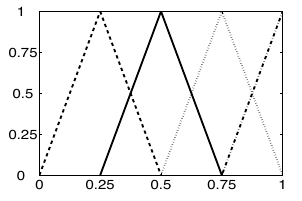
\includegraphics[width=\textwidth]{figures/ArbogastCoarse} \\
      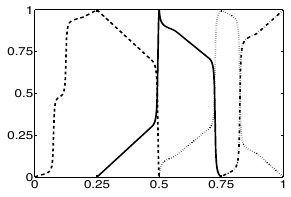
\includegraphics[width=\textwidth]{figures/ArbogastCoarseMs} \\
      {\small [Arbogast 2011]}
    \end{column}
    \begin{column}{0.6\textwidth}
      \begin{itemize}
      \item subassembly avoids explicit matrix triple product $A_{\text{coarse}} \gets P^T A_{\text{fine}} P$
      \item can update the coarse operator locally (e.g.~local nonlinearity)
      \item need not assemble entire fine grid operator
      \item if repetitive structure, need not store entire fine grid state
      \item can coarsen very rapidly (especially in smooth regions)
      \item lower communication setup phase
      \end{itemize}      
    \end{column}
  \end{columns}
\end{frame}
